\usetikzlibrary{arrows.meta, positioning}
\begin{figure*}
  \centering
  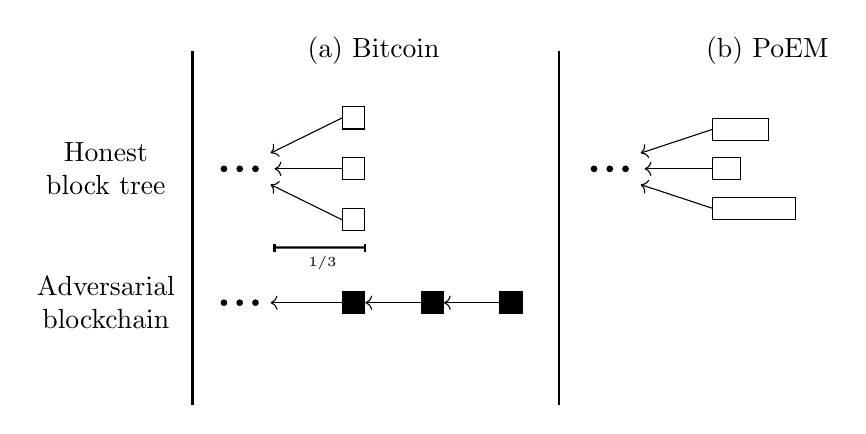
\begin{tikzpicture}

  % Define styles
  \tikzstyle{dot} = [circle, draw, fill=black, minimum size=2pt, inner sep=0pt]
  \tikzstyle{block} = [rectangle, draw, minimum size=8pt]
  \tikzstyle{adv_block} = [rectangle, draw, fill=black, minimum size=8pt]
  \tikzstyle{dashed_line} = [draw, dashed, thick]

  % Labels
  \node at (1.4, 5.5) {(a) Bitcoin};
  \node[align=center] at (-2, 4) {Honest \\ block tree};
  \node[align=center] at (-2, 2.3) {Adversarial \\ blockchain};

  \draw[thick] (-0.9, 1) -- (-0.9, 5.5);

  % Bitcoin Honest
  \node[dot, fill] (dot1) at (-0.5, 4) {};
  \node[dot] (dot2) at (-0.3, 4) {};
  \node[dot] (dot3) at (-0.1, 4) {};

  \node[block, anchor=west] (h2) at (1, 4) {};
  \node[block, anchor=west] (h1) [above=10pt of h2] {};
  \node[block, anchor=west] (h3) [below=10pt of h2] {};

  % Honest tree connections
  \draw[<-] (dot3.east) ++(0.15,0.2) -- (h1.west);
  \draw[<-] (dot3.east) ++(0.2,0) -- (h2.west);
  \draw[<-] (dot3.east) ++(0.15,-0.2) -- (h3.west);

  % Bitcoin Adversary
  \node[dot, fill] (dot1) at (-0.5, 2.3) {};
  \node[dot] (dot2) at (-0.3, 2.3) {};
  \node[dot] (dot3) at (-0.1, 2.3) {};

  \node[adv_block, anchor=west] (a1) at (1, 2.3) {};
  \node[adv_block, anchor=west] (a2) [right=20pt of a1] {};
  \node[adv_block, anchor=west] (a3) [right=20pt of a2] {};

  % Adversarial chain connections
  \draw[<-] (dot3.east) ++(0.15,0) -- (a1.west);
  \draw[<-] (a1) -- (a2);
  \draw[<-] (a2) -- (a3);

  % Bracket for Bitcoin (2/3)
  \draw[thick] (dot3.east) ++(0.2,0.7) -- ([xshift=0.0cm,yshift=0.7cm]a1.east) ++(0,-0.5);
  \draw[thick] (dot3.east) ++(0.2,0.75) -- ([xshift=0.2cm,yshift=0.65cm]dot3.east) ++(0,-0.2);
  \draw[thick] (a1.east) ++(0.0,0.75) -- ([xshift=0.0cm,yshift=0.65cm]a1.east) ++(0,-0.2);
  \node at (0.75, 2.8) {\tiny 1/3};


  % PoEM Section
  % Labels
  \node at (6.4, 5.5) {(b) PoEM};

  \draw[thick] (3.75, 1) -- (3.75, 5.5);
  % PoEM Honest
  \node[dot, fill] (dot3) at (4.6, 4) {};
  \node[dot] (dot2) at (4.4, 4) {};
  \node[dot] (dot1) at (4.2, 4) {};

  \node[block, minimum width=10pt, anchor=west] (h2) at (5.7, 4) {};
  \node[block, minimum width=20pt, anchor=west] (h1) at (5.7, 4.5) {};
  \node[block, minimum width=30pt, anchor=west] (h3) at (5.7, 3.5) {};

  % Honest tree connections
  \draw[<-] (dot3.east) ++(0.15,0.2) -- (h1.west);
  \draw[<-] (dot3.east) ++(0.2,0) -- (h2.west);
  \draw[<-] (dot3.east) ++(0.15,-0.2) -- (h3.west);


  \end{tikzpicture}
  \caption{A Bitcoin (left) and a PoEM (right) execution where the honest parties (top) and the adversary (bottom)
           are handed the same blocks. The honest Bitcoin tree grows faster than the honest PoEM tree as compared
           to the adversarial chain.}
  \label{fig:poem-wasted-work}
\end{figure*}